%%%%%% Algorithms
To apply multigrid efficiently for the SBP-SAT method on GPUs, we need to develop a new geometric multigrid formulation that does not require using algebraic coarsening or Galerkin's condition.

Matrix-free iterative methods enable the solution to larger problems compared to a direct solve that requires storing a matrix factorization.  However, the convergence of CG depends predominantly on the condition number and quality of the initial guess. The condition number can be reduced through preconditioning techniques, but the preconditioning matrix $\mathbf{M}$ has to be SPD and fixed, and although it need not be explicitly assembled nor inverted, good preconditioners should satisfy $\mathbf{M} \approx \mathbf{A}^{-1}$. 


To our knowledge, preconditioning has not been explored for CG methods applied to SBP-SAT discretizations. 
% Existing work using multigrid as a solver for problems with SBP-SAT methods focused on using SBP-preserving interpolation operators with the Galerkin coarsening to build the coarse grid operators 
Existing work using multigrid as a solver for problems with SBP-SAT methods focused on using SBP-preserving interpolation operators with the Galerkin coarsening to build the coarse grid operators \citep{Ruggiu2018}. Here the standard interpolation operators were modified for boundary points to preserve the SBP property \citep{Ruggiu2018}. However, although Galerkin coarsening or other algebraic multigrid methods produce coarse grid operators automatically (and therefore can be seen as a ``plug-in" solver for any linear system \citep{stuben2001review}), defining these matrix-free coarse grid operators in this fashion requires writing a different kernel for every grid level, as well as more memory for data storage \citep{brandt2006guide}. 
Moreover, it also increases overhead in pre-compiling matrix-free kernels for different $N$s due to the just-in-time (JIT) compiling mechanism in Julia. Therefore, to fully utilize the efficiency of our matrix-free methods, as well as to reduce complexity in and number of kernels needed, developing geometric multigrid preconditioned CG (denoted MGCG) for the SBP-SAT method becomes the key focus of our work. 

Three key ingredients define multigrid methods, namely, interpolation operators (prolongation and restriction), smoothers, and (if used) a direct solve on a coarse grid.  In this work we adopt the second-order SBP-preserving prolongation/restriction operators from \citep{Ruggiu2018}, which maintain accuracy at domain boundaries and correctly transfer residual vectors to the coarser grids. The 2D restriction operator is given by

\begin{equation}
    \boldsymbol{I}_{h}^{2h} = \boldsymbol{H}_{2h}^{-1} \left(\boldsymbol{I}_{2h}^h\right)^T\boldsymbol{H}_h
\end{equation}
%
where $\boldsymbol{H}_{h}$ and $\boldsymbol{H}_{2h}$ denote $\boldsymbol{H} \otimes \boldsymbol{H}$ with grid spacing $h$ and $2h$, respectively. The 2D prolongation operator $\boldsymbol{I}_{2h}^h$ is defined by $\boldsymbol{I}_{2h}^h = I_{2h}^h \otimes I_{2h}^h$, where $I_{2h}^h$ is the standard 1D prolongation operator \citep{10.5555/357695}, see Appendix A in \citep{Ruggiu2018}.

One feature that differentiates our problem formulation from those in \citep{Ruggiu2018} is that our matrix in SBP-SAT methods is rendered SPD only after the multiplication of \eqref{eqn: D2} on the left by $\left(\boldsymbol{H} \otimes \boldsymbol{H} \right)$, which introduces additional grid information when calculating the associated residual vector. To properly transfer this grid information we found improved performance when further modifying the restriction operator to account for grid spacing. This is achieved by excluding the $\left(\boldsymbol{H} \otimes \boldsymbol{H} \right)$ term when computing the residual on the fine grid, then restricting using $\boldsymbol{I}_r$, and then re-introducing the grid spacing on the coarse grid. This process requires ``applying" the inverse: Given that $\left(\boldsymbol{H} \otimes \boldsymbol{H} \right)$ is a sparse diagonal matrix (thus its inverse is the diagonal matrix of reciprocal values), GPU kernels for the multiplication of this matrix and its inverse can be easily implemented in a matrix-free manner. The pseudo-code for the geometric multigrid method is given in Algorithm \autoref{alg:mg-modified}.





\begin{algorithm*}
    \caption{$(k+1)$-level MG for $\boldsymbol{A}_h \boldsymbol{u}_h = \boldsymbol{f}_h$, with smoothing $S_{h_k}^{\nu}$ applied $\nu$ times. SBP-preserving restriction and interpolation operators are applied. Grid coarsening ($k \to k+1$) is done through successive doubling of grid spacing until reaching the coarsest grid. The multigrid cycle can be performed $N_{maxiter}$ times. $\boldsymbol{r}$ represents the residual, and $\boldsymbol{v}$ represents the solution to the residual equation used during the correction step. This algorithm is adapted from \citep{liu2023multigrid}.}\label{alg:mg-modified}
    \algrenewcommand\algorithmicprocedure{\textbf{function}}
    \begin{algorithmic}
    \Procedure{MG}{$\boldsymbol{f}_{h_k}$, $\boldsymbol{A}_{h_k}$, $\boldsymbol{u}_{h_k}^{(0)}$, $k$, $N_{maxiter}$}
    \For {$n = 0, 1, 2, \dots, N_{maxiter}$} 
                
        \State $\boldsymbol{u}_{h_k}^{(n)}$ $\xleftarrow[]{S_{h_k}^{\nu_1}}$ $\boldsymbol{u}_{h_k}^{(n)}$ \Comment{Pre-smoothing $\nu_1$ times}
        \State  $\boldsymbol{r}_{h_k}^{(n)} = \boldsymbol{f}_{h_k}^{(n)} - \boldsymbol{A}_{h_k}^{(n)} \boldsymbol{u}_{h_k}^{(n)}$ \Comment{Calculating residual}
        \State  $\tilde{\boldsymbol{r}}_{h_{k}} =  (\boldsymbol{H}_k \otimes \boldsymbol{H}_k)^{-1} \boldsymbol{r}_{h_k}^{(n)}$  \Comment{Removing grid info}
    
        \State     $\boldsymbol{r}_{h_{k+1}} = (\boldsymbol{H}_{k+1} \otimes \boldsymbol{H}_{k+1}) \boldsymbol{I}_{h_{k}}^{h_{k+1}} \tilde{\boldsymbol{r}}_{h_{k}}$ \Comment{Restriction}
        \If{$k + 1 = k_\text{max}$}
        \State $\boldsymbol{v}_{h_{k+1}}^{(n)}$ $\xleftarrow[]{S_{h_{k+1}}^{\nu_2}}$ $\boldsymbol{0}_{h_{k+1}}^{}$ 
                    \Comment{Smoothing on coarsest grid}
        \Else
        \State $\boldsymbol{v}_{h_{k+1}}^{(n)}$ = MG({$\boldsymbol{r}_{h_{k+1}}$, $\boldsymbol{A}_{h_{k+1}}$, $\boldsymbol{0}_{h_{k+1}}^{}$, $k + 1$, $1$})
        \State       \Comment{Recursive definition of MG}   
        \EndIf
        \State  $\boldsymbol{v}_{k}^{n} = \boldsymbol{I}_{h_{k+1}}^{h_k} \boldsymbol{v}_{k+1}^{(n)}$
                 \Comment{Interpolation}
        \State $\boldsymbol{u}_{k}^{(n+1)} = \boldsymbol{u}_{k}^{(n)} + \boldsymbol{v}_{k}^{n}$ \Comment{Correction}
        \State   $\boldsymbol{u}_{k}^{(n+1)} \xleftarrow[]{S_{h_k}^{\nu_3}}$ $\boldsymbol{u}_{h_k}^{(n+1)}$ \Comment{Post-smoothing $\nu_3$ times}
    \EndFor
    \EndProcedure
    % \Require
    \end{algorithmic}
\end{algorithm*}






Many types of smoothers for multigrid methods can be explored for best performance.  In this work we choose the Richardson iteration given by $\mathbf{x}_{k+1} = \mathbf{x}_k + \omega (\mathbf{b} - \mathbf{A}\mathbf{x}_k)$
because it can be easily implemented with our existing matrix-free kernel. Here $\omega$ is chosen to satisfy the convergence criteria and its optimal value depends on the eigenvalues of $\boldsymbol{A}$ as $\omega_{opt} = \frac{2}{\lambda_{max} + \lambda_{min}}$, where $\lambda_{max}$ and $\lambda_{min}$ are the largest and smallest eigenvalues of $\boldsymbol{A}$ respectively.
We use Arpack.jl, which is a Julia wrapper of ARPACK that uses the Implicitly Restarted Arnoldi Method to calculate eigenvalues for sparse matrices.
For small $N$, we can compute $\lambda_{max}$ and $\lambda_{min}$ directly, but for large $N$ values, these become computationally intractable. We use interpolation to approximate values for $\lambda_{max}$ and $\lambda_{min}$ for $N \geq 32$ based on observation of eigenvalues for $N \leq 32$, namely,
%
\begin{align*}
    \lambda_{min, 2N} &= \lambda_{min, N} / 4, \\
    \lambda_{max, 2N} &= \lambda_{max, N} + 0.6 * (\lambda_{max, N} - \lambda_{max, N/2}),
\end{align*}
where $\lambda_{min, N}$ represents the minimal eigenvalue of a linear system formed for our 2D problem with $N+1$ grid points in each direction and $\lambda_{max, N}$ is the corresponding maximum value.
In practice, these interpolated eigenvalues provide a relatively tight lower and upper bound for the real eigenvalues and appear to be sufficient according to our performance results.
Alternative smoothers could be considered, such as Jacobi iteration or SSOR, but these require the decomposition of the linear system and the development of additional GPU kernels. 
We did test these smoothers in experiments using the matrix-explicit formulation and found that they perform at similar levels to the Richardson iteration when multigrid is used as a preconditioner. We found that the total number of iterations required by MGCG is largely determined by the number of grid levels and smoothing steps and is less impacted by the choice of smoother itself. 
%
\begin{figure}[t]
    \centering
    %\includegraphics[width=\textwidth]{sparsity_patter_A.png}
    %  \includegraphics[width=0.8\textwidth]{mgcg_richardson.pdf}
    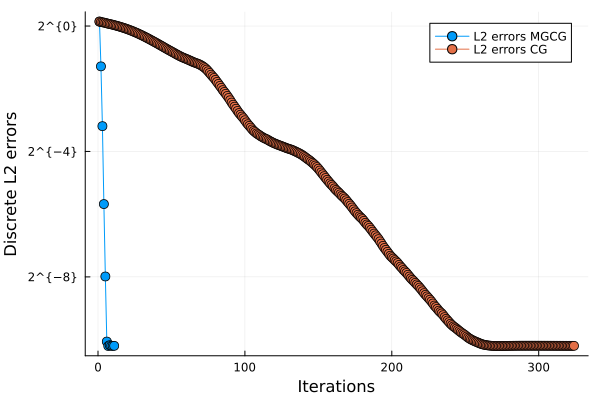
\includegraphics[width=\linewidth]{figures/64_L2_errors.png}
    \caption{Log of error (difference from a direct solve) versus iteration count for multigrid preconditioned conjugate gradient (MGCG), shown in blue circles, using 5 steps of pre- and post-Richardson smoothing for every level versus unpreconditioned conjugate gradient (CG), shown in orange circles, for $N = 2^5$.}
    \label{fig:mgcg_conv}
\end{figure}
%
%



Multigrid methods have many tunable parameters. For this initial study, we implemented MGCG with 5 Richardson pre- and  post-smoothing steps on every level with a single V-cycle (i.e. taking $\nu_1 = \nu_2 = \nu_3 = 5$ and $N_{maxiter} = 1$ in Algorithm 1), including on the coarsest grid (5 grid points in each direction). This avoids using a direct solve on the coarse grid which would require conversion between CPU arrays and GPU arrays.
All operations in this MGCG algorithm can be implemented in a matrix-free manner in a way that does not require storing matrix $\boldsymbol{A}$ on any grid level.  
% We compare our matrix-free MGCG (denoted MF-MGCG) algorithm against the standard, non-preconditioned CG algorithm implemented with cuSPARSE. 

% The results are given Table \ref{tab:mgcg}. Our matrix-free implementation beats SpMV consistently whether or not we use preconditioning. We also see that the MGCG algorithms beat the direct solve consistently for both matrix-free and SpMV implementations.  As $N$ doubles, the number of iteration steps for MGCG stays at the same level $\sim$10.

% The MGCG requires a relatively constant number of iterations to converge as $N$ is doubled, but CG requires 2$\times$ more iteration steps when $N$ is doubled, presumably due to an increase in condition number.
To show the drastically different behaviors, we plot the discrete $\mathit{L}^2$-error against iteration counts for $N = 32$ for CG and MGCG in \autoref{fig:mgcg_conv}.
MGCG converges after only $\sim$5 iterations. Additional iterations are coming from the additional discrete $\mathit{L}^2$-error requirement in the stopping criteria.
Since the complexity of each CG iteration step is $\mathcal{O}(N^2)$, as $N$ doubles the total time increases by a factor of 4 for MGCG versus 8 for CG. 
% The number of degrees of freedom quadruples when $N$ is doubled. As a result, the total throughput in degrees of freedom remains at the same level of magnitude for MGCG methods, but the CG and direct solve see memory throughput reduced by roughly 2$\times$ when $N$ doubles, see Table \ref{tab:DOF}. Memory throughput drops for $N=2^{13}$ as compared to $N=2^{12}$ for the MF-MGCG due to the increased iteration count. 
% This is because of the $\mathit{L}^2$-error used in the stopping criterion. For MGCG using only the residual stopping criterion, the peak performance for $N=2^{13}$ is above $70$ MDoF/s.
In this section we present a new formulation multigrid preconditioned conjugate gradient that can be implemented matrix-free with a Richardson smoother in order to solve 2D, variable coefficient elliptic problems discretized with an SBP-SAT method. 

%We show that matrix-free kernels outperform the cuSPARSE SpMV kernels from NVIDIA in both runtime and memory usage.
% The MGCG algorithm achieves nearly constant iteration steps to converge for various problem sizes, reducing iteration steps by up to $4000\times$ and total runtime by up to $600\times$.


